\documentclass[12pt,a4paper,english]{article}

\usepackage[pdftex]{graphicx}
\usepackage[utf8]{inputenc}
\usepackage[hyphens]{url}
\usepackage[unicode, colorlinks=true, hypertexnames=false, allcolors=red, linkcolor=blue]{hyperref}
\usepackage{xcolor}
\usepackage{times}
\usepackage{amsmath}


\newcommand{\todo}[1]{\textcolor{red}{[[\textbf{TODO} \textbf{#1]]}}}

\begin{document}
    \begin{titlepage}
        \begin{center}
            \vspace*{1cm}
        
            \begin{figure}[h!]
                
\includegraphics[scale=0.12]{VUT-FIT-logo-en.png}
            \end{figure}
            \vspace{1.5cm}

            \Large{\textbf{Epidemiological models - macro level model}} \\
            \large{Modelling and Simulation}

            \vspace{0.5cm}
                
            \vspace{1.5cm}
            
            \textbf{Abramov Mikhail (xabram00)} \\
            \textbf{Pavel Yadlouski (xyadlo00)} 

            \vfill
                
            \vspace{0.8cm}
        
            Brno University of Technologies\\
            November, 2020
                
        \end{center}
    \end{titlepage}

    \tableofcontents
    \newpage

    \section{Introduction}
    The first aim is to determine the possibilities for determining the value of the effectiveness of various restrictive measures taken by the government of the Czech Republic for the period from September 1, 2020 till the last day of the project - December 7, 2020.

    The second aim is to create a predictive model for determining the number of persons who have illness in the same time, persons who have been ill or otherwise have immunity
    % \todo{перенести это в пункт с допущениями когда он будет?}, the number persons who will not be able to resist the disease and as a result will die. 
    % \todo{Данные показатели очень важны для принятия решения о: 1) вводе новых мер 2) отмене старых мер 3) подготовке больничных мест, т.к. при их нехватке смертность значительно возрастает 4) оценка последствий как мер так и самой болезни}
    
    Used model contains different scenarios of quarantine precautions (using different types of lockdown).
    Based on simulations of this scenarios, influence of particular scenario is shown. 
    As an experiment, theoretical scenarios from the article and current lockdown type in Czech Republic are analyzed.

    \subsection{Contributors}    
    This project is solved by team of two students: Abramov Mikhail and Pavel 
    Yadlouski.

    \subsection{Model validation}
    Results of theoretical scenarios simulation are compared with reference results from the article. 
    The article by itself was subjected to critical analysis and minor formulas adjustments.
    Experiment with lockdown type in Czech Republic is compared with reality:) 
    
    % \todo{Для достижения поставленных задач было выбрано исследование - ссылочка. Данная статья использует модифицированную модель СИРД для оценки изучения и оценки различных моделей карантинных мер. 
    %       Данная модель без модификаций имеет довольно широкое распространенние и часто используется для описания распространения заболеваний. (можно бахнуть несколько других статей как подтверждение что модель часто импользуется)
    %       Валидация корректности имплементации данной модели была сверена с результатами представленными в статье а сама статья подвержена критическому анализу и незначительной корректировке формул. <- DONE
    %       Далее для определения эффективности мер принятых чешским правительство (надо накидать ссылочек на меры мб) использовалась модель подготовленная в соответствии с приведенной выше статьей и статистика по заболеванию Ковид из официальных источников (ссылочка на ковид стат).
    %       За валидацию корректности наших гипотетических оценок принято соответствие основных трендов развития модели с данныими официальной статистики}.
    
    \section{Topic analysis}
    The necessary information to research this topic was found in scientific articles from IRCACS-International Research Center for Applied Complexity Sciences in  Colombia written by Danny Ibarra-Vega\cite{math_article}

    As epidemic situation in the world become worth with time, there is need to take appropriate precautions based on mathematical models and simulation. 
    One of the base mathematical model for simulation of expansion of the epidemic is SIR model. 
    SIR\footnote{https://en.wikipedia.org/wiki/Compartmental\_models\_in\_epidemiology} model is one of the simplest compartment methods.
    \newpage
    \noindent This method compares three values:
    \begin{enumerate}
        \item \textbf{S} -- the number of \textbf{s}usceptible individuals
        \item \textbf{I} -- the number of \textbf{i}nfectious individuals.
        \item \textbf{R} -- the number of \textbf{r}emoved (and immune) or deceased individuals
    \end{enumerate} 

    \subsection{Approaches}
    For more complex view of system behavior, a mathematical model has been adopted with the Systems Dynamics(SD) methodology\footnote{https://en.wikipedia.org/wiki/System\_dynamics}.
    The core of this methodology is that SD models solve the problem of simultaneity (mutual causation) by updating all variables in small time increments with positive and negative feedbacks and time delays structuring the interactions and control.
    
    Used SD model extends basic SIR model with separating the number of recovered and deceased individuals into two variables and addition of auxiliary and state variables that represent hospital capacity, contacts, contacts with infected. 
    As a result, there is a model of 4 stock variables (\ref{conc_model}).
    
    \subsection{Sources}
    Article with the mathematical model \cite{math_article} for implementation is 
    found in VUT online library \footnote{https://www-sciencedirect-com.ezproxy.lib.vutbr.cz}

    \section{Concept model} \label{conc_model}
    In the model, we proceed from the assumption that immunity is stable and guarantees the absence of recurrent disease for the duration of research period. 
    
    \newpage
    Following diagram taken from the reference article. 
    
    \begin{figure}[ht!]
        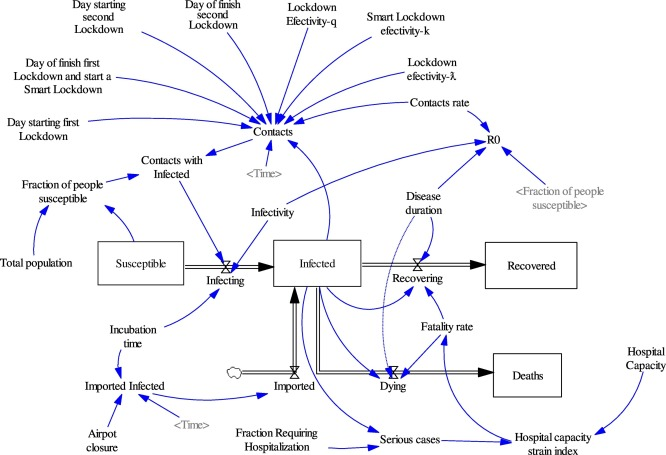
\includegraphics[scale=0.85]{1-s2.0-S0048969720324347-gr1.jpg}
        \caption[]{Stock and flows diagram \cite{math_article}}
        \label{fig:graph}
    \end{figure}

    It shows how each stock (susceptible, infectious, removed, deaths) variable is connected and influenced by other stock and auxiliary variable. 
    Auxiliary variables are constructed from bibliographic references or some estimated, as shown in the  

    \begin{table}
        
    \end{table}
    Mathematical equations:
        \begin{align*}
            \frac{dS}{dt} &= - \frac{\beta Ci}{it}\\ \\
            \frac{dI}{dt} &= \frac{\beta C}{it} - \frac{I}{Dd} * (1 - Fr)\\ \\
            \frac{dR}{dt} &= \frac{I}{Dd} * (1 - Fr)\\ \\
            \frac{dD}{dt} &= \frac{I}{Dd} * (Fr)
        \end{align*}        
    \section{Experiment}
    
    \todo{Misha napishy suda}

    \section{Conclusion}
    \todo{Co se naucili}
    
    \todo{Doporuceni}

    \todo{Experiment with other country}

    \clearpage
	\bibliographystyle{abbrv}
	\bibliography{citation}
\end{document}